% Generated by pysimcount.pfchilds -- do not edit; regenerate instead.
% figure: optimised-cnot-all-formulas -- Every formula, Nam Light optimised step, cnot gates vs n
% source: ../np-optimised-seeds/aggregate.json (seeds [1, 2, 3, 4, 5, 6, 7, 8, 9, 10]); run commits: e42ff29056ad9ea7fc7c9899fab334903e42e3e3
% metric=cnot kind=optimised merged (cz, simcount template)
% measured n: mean over seeds of the run's totals; bars min..max over seeds
% r from power-law fit to mean measured r (n = 5--10); r = ceil(a n^b); point=mean-r-fit; bars = min..max of per-seed fits
% per-step counts exactly affine in n (checked on n = [10, 13, 16])
% n > 16: optimised per-step count from linear fit (n = 10--16); circuit not built or verified
% shown: suzuki4, suzuki6, mo-q6, mo-q14, bm-q10, mo-o8-q21, morales-y8m10, morales-m8
% removed (see optimised-cnot-all-formulas-ranking.md): lie-trotter, suzuki2, suzuki8
% figure made at git_commit=e5d9ee696f892e28aced765585653760f8a427c4 git_dirty=False
% derived: optimised-cnot-all-formulas.tex restyled by pysimcount.figuniform: extrapolated points (r from power-law fit) drawn in their series' measured style, style-key legend entries removed; extrapolated n = [13, 20, 30, 50, 70, 100, 200, 300, 500]; source_sha256=76d4c9dc5ef196e36973b097db39f656e64c96710ea30d621505e8184f6d9e95
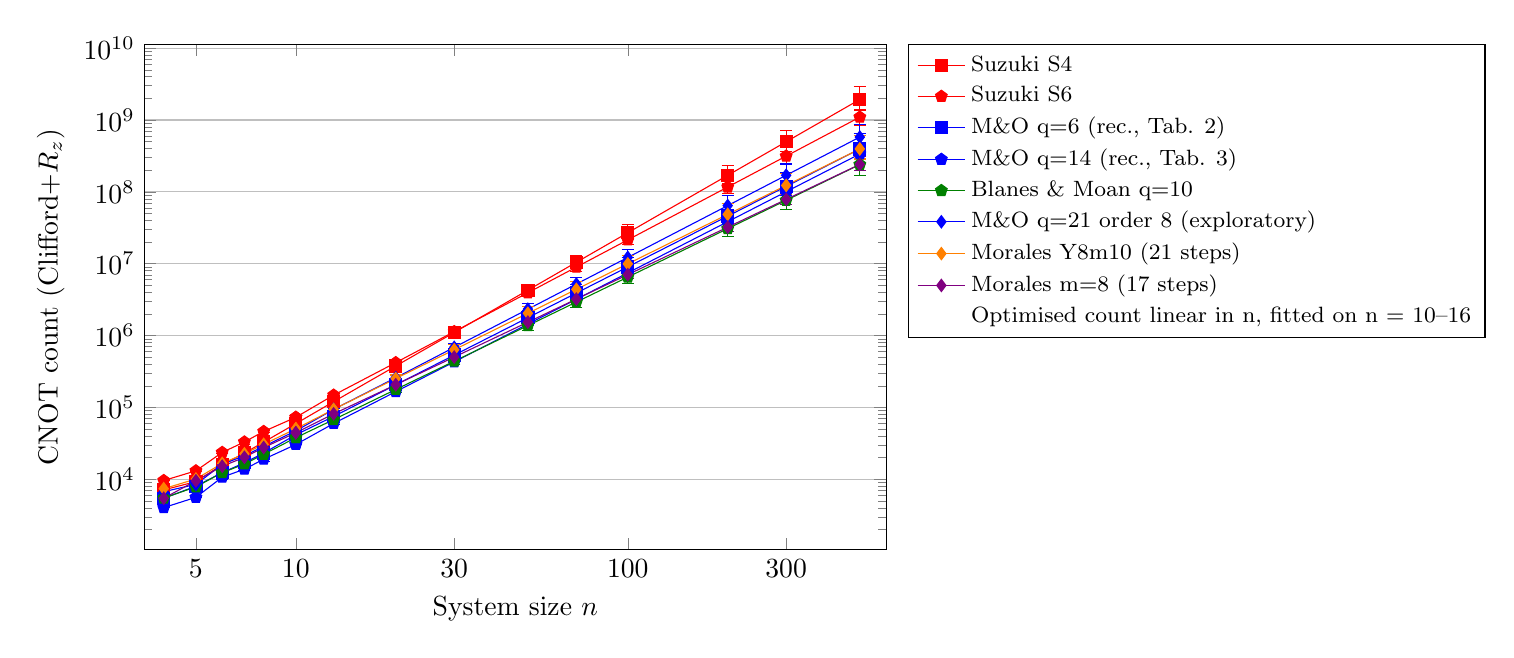
\begin{tikzpicture}
  \begin{loglogaxis}[
    width=11cm, height=8cm,
    xlabel={System size $n$},
    ylabel={CNOT count (Clifford+$R_z$)},
    xtick={5,10,30,100,300}, xticklabels={5,10,30,100,300},
    xmin=3.5, xmax=600,
    ymajorgrids=true,
    legend pos=outer north east,
    legend cell align=left,
    legend style={font=\footnotesize},
  ]
    % suzuki4: measured n, mean over seeds, bars min..max over seeds
    \addplot[red, solid, mark=square*, mark size=2.2pt, mark options={solid, fill=red}, error bars/.cd, y dir=both, y explicit, error bar style={solid}] coordinates {
      (4,7104) += (0,96) -= (0,64)
      (5,9280) += (0,320) -= (0,280)
      (6,15912) += (0,1128) -= (0,792)
      (7,23128) += (0,1792) -= (0,1568)
      (8,32896) += (0,1344) -= (0,1216)
      (10,59440) += (0,4560) -= (0,2240)
    };
    \addlegendentry{Suzuki S4}
    % suzuki4: extrapolated, r = ceil(3.30875 n^1.65448), per step = 40 n + 0; bars min..max of per-seed fits
    \addplot[red, solid, mark=square*, mark size=2.2pt, mark options={solid, fill=red}, forget plot, error bars/.cd, y dir=both, y explicit, error bar style={solid}] coordinates {
      (10,59440)
      (13,120120) += (0,7280) -= (0,6760)
      (20,376800) += (0,40000) -= (0,32800)
      (30,1.104e+06) += (0,168000) -= (0,126000)
      (50,4.282e+06) += (0,906000) -= (0,634000)
      (70,1.04608e+07) += (0,2.6348e+06) -= (0,1.778e+06)
      (100,2.696e+07) += (0,7.988e+06) -= (0,5.192e+06)
      (200,1.69736e+08) += (0,6.5704e+07) -= (0,3.984e+07)
      (300,4.97976e+08) += (0,2.20668e+08) -= (0,1.28652e+08)
      (500,1.9324e+09) += (0,9.9904e+08) -= (0,5.547e+08)
    };
    % suzuki6: measured n, mean over seeds, bars min..max over seeds
    \addplot[red, solid, mark=pentagon*, mark size=2.2pt, mark options={solid, fill=red}, error bars/.cd, y dir=both, y explicit, error bar style={solid}] coordinates {
      (4,9600) += (0,0) -= (0,0)
      (5,13100) += (0,900) -= (0,100)
      (6,23640) += (0,1560) -= (0,840)
      (7,33040) += (0,1960) -= (0,2240)
      (8,46240) += (0,1760) -= (0,1440)
      (10,72800) += (0,5200) -= (0,2800)
    };
    \addlegendentry{Suzuki S6}
    % suzuki6: extrapolated, r = ceil(1.3813 n^1.44491), per step = 200 n + 0; bars min..max of per-seed fits
    \addplot[red, solid, mark=pentagon*, mark size=2.2pt, mark options={solid, fill=red}, forget plot, error bars/.cd, y dir=both, y explicit, error bar style={solid}] coordinates {
      (10,72800)
      (13,148200) += (0,7800) -= (0,5200)
      (20,420000) += (0,48000) -= (0,24000)
      (30,1.134e+06) += (0,180000) -= (0,90000)
      (50,3.94e+06) += (0,880000) -= (0,420000)
      (70,8.974e+06) += (0,2.366e+06) -= (0,1.134e+06)
      (100,2.144e+07) += (0,6.68e+06) -= (0,3.14e+06)
      (200,1.1672e+08) += (0,4.752e+07) -= (0,2.148e+07)
      (300,3.1458e+08) += (0,1.4646e+08) -= (0,6.462e+07)
      (500,1.0967e+09) += (0,5.96e+08) -= (0,2.538e+08)
    };
    % mo-q6: measured n, mean over seeds, bars min..max over seeds
    \addplot[blue, solid, mark=square*, mark size=2.2pt, mark options={solid, fill=blue}, error bars/.cd, y dir=both, y explicit, error bar style={solid}] coordinates {
      (4,5433.6) += (0,326.4) -= (0,633.6)
      (5,8016) += (0,384) -= (0,816)
      (6,12355.2) += (0,316.8) -= (0,547.2)
      (7,16968) += (0,840) -= (0,1176)
      (8,23193.6) += (0,2150.4) -= (0,1305.6)
      (10,41568) += (0,1632) -= (0,2688)
    };
    \addlegendentry{M\&O q=6 (rec., Tab. 2)}
    % mo-q6: extrapolated, r = ceil(3.76178 n^1.34927), per step = 48 n + 0; bars min..max of per-seed fits
    \addplot[blue, solid, mark=square*, mark size=2.2pt, mark options={solid, fill=blue}, forget plot, error bars/.cd, y dir=both, y explicit, error bar style={solid}] coordinates {
      (10,41568)
      (13,74880) += (0,6864) -= (0,3744)
      (20,206400) += (0,28800) -= (0,16320)
      (30,534240) += (0,103680) -= (0,57600)
      (50,1.7712e+06) += (0,472800) -= (0,247200)
      (70,3.90432e+06) += (0,1.23312e+06) -= (0,631680)
      (100,9.024e+06) += (0,3.3408e+06) -= (0,1.6608e+06)
      (200,4.59648e+07) += (0,2.21856e+07) -= (0,1.03488e+07)
      (300,1.19146e+08) += (0,6.58368e+07) -= (0,2.95776e+07)
      (500,3.95592e+08) += (0,2.57448e+08) -= (0,1.09368e+08)
    };
    % mo-q14: measured n, mean over seeds, bars min..max over seeds
    \addplot[blue, solid, mark=pentagon*, mark size=2.2pt, mark options={solid, fill=blue}, error bars/.cd, y dir=both, y explicit, error bar style={solid}] coordinates {
      (4,4032) += (0,0) -= (0,0)
      (5,5600) += (0,0) -= (0,0)
      (6,10684.8) += (0,67.2) -= (0,604.8)
      (7,13798.4) += (0,313.6) -= (0,470.4)
      (8,18995.2) += (0,716.8) -= (0,1075.2)
      (10,30464) += (0,896) -= (0,224)
    };
    \addlegendentry{M\&O q=14 (rec., Tab. 3)}
    % mo-q14: extrapolated, r = ceil(1.21616 n^1.36863), per step = 112 n + 0; bars min..max of per-seed fits
    \addplot[blue, solid, mark=pentagon*, mark size=2.2pt, mark options={solid, fill=blue}, forget plot, error bars/.cd, y dir=both, y explicit, error bar style={solid}] coordinates {
      (10,30464)
      (13,59696) += (0,2912) -= (0,1456)
      (20,165760) += (0,11200) -= (0,4480)
      (30,430080) += (0,43680) -= (0,13440)
      (50,1.4448e+06) += (0,179200) -= (0,61600)
      (70,3.19872e+06) += (0,462560) -= (0,148960)
      (100,7.448e+06) += (0,1.232e+06) -= (0,403200)
      (200,3.8416e+07) += (0,8.0192e+06) -= (0,2.4864e+06)
      (300,1.00397e+08) += (0,2.34192e+07) -= (0,7.1568e+06)
      (500,3.3656e+08) += (0,8.9544e+07) -= (0,2.6712e+07)
    };
    % bm-q10: measured n, mean over seeds, bars min..max over seeds
    \addplot[green!50!black, solid, mark=pentagon*, mark size=2.2pt, mark options={solid, fill=green!50!black}, error bars/.cd, y dir=both, y explicit, error bar style={solid}] coordinates {
      (4,5472) += (0,288) -= (0,32)
      (5,7840) += (0,160) -= (0,240)
      (6,12336) += (0,144) -= (0,336)
      (7,16296) += (0,504) -= (0,616)
      (8,22272) += (0,1408) -= (0,1152)
      (10,37920) += (0,480) -= (0,1120)
    };
    \addlegendentry{Blanes \& Moan q=10}
    % bm-q10: extrapolated, r = ceil(2.67799 n^1.24119), per step = 80 n + 0; bars min..max of per-seed fits
    \addplot[green!50!black, solid, mark=pentagon*, mark size=2.2pt, mark options={solid, fill=green!50!black}, forget plot, error bars/.cd, y dir=both, y explicit, error bar style={solid}] coordinates {
      (10,37920)
      (13,67600) += (0,3120) -= (0,3120)
      (20,177600) += (0,14400) -= (0,14400)
      (30,439200) += (0,50400) -= (0,48000)
      (50,1.376e+06) += (0,216000) -= (0,196000)
      (70,2.9288e+06) += (0,532000) -= (0,487200)
      (100,6.512e+06) += (0,1.376e+06) -= (0,1.232e+06)
      (200,3.0768e+07) += (0,8.384e+06) -= (0,7.152e+06)
      (300,7.632e+07) += (0,2.364e+07) -= (0,1.9584e+07)
      (500,2.398e+08) += (0,8.576e+07) -= (0,6.86e+07)
    };
    % mo-o8-q21: measured n, mean over seeds, bars min..max over seeds
    \addplot[blue, solid, mark=diamond*, mark size=2.2pt, mark options={solid, fill=blue}, error bars/.cd, y dir=both, y explicit, error bar style={solid}] coordinates {
      (4,6720) += (0,0) -= (0,0)
      (5,8484) += (0,756) -= (0,84)
      (6,16128) += (0,1008) -= (0,1008)
      (7,21285.6) += (0,1058.4) -= (0,1293.6)
      (8,28627.2) += (0,940.8) -= (0,1747.2)
      (10,47208) += (0,3192) -= (0,1848)
    };
    \addlegendentry{M\&O q=21 order 8 (exploratory)}
    % mo-o8-q21: extrapolated, r = ceil(1.17031 n^1.39675), per step = 168 n + 0; bars min..max of per-seed fits
    \addplot[blue, solid, mark=diamond*, mark size=2.2pt, mark options={solid, fill=blue}, forget plot, error bars/.cd, y dir=both, y explicit, error bar style={solid}] coordinates {
      (10,47208)
      (13,93912) += (0,4368) -= (0,4368)
      (20,258720) += (0,26880) -= (0,20160)
      (30,685440) += (0,95760) -= (0,75600)
      (50,2.3268e+06) += (0,462000) -= (0,336000)
      (70,5.20968e+06) += (0,1.2348e+06) -= (0,870240)
      (100,1.22304e+07) += (0,3.4776e+06) -= (0,2.3184e+06)
      (200,6.43776e+07) += (0,2.42592e+07) -= (0,1.49856e+07)
      (300,1.701e+08) += (0,7.3836e+07) -= (0,4.36464e+07)
      (500,5.78592e+08) += (0,2.94672e+08) -= (0,1.65396e+08)
    };
    % morales-y8m10: measured n, mean over seeds, bars min..max over seeds
    \addplot[orange, solid, mark=diamond*, mark size=2.2pt, mark options={solid, fill=orange}, error bars/.cd, y dir=both, y explicit, error bar style={solid}] coordinates {
      (4,7392) += (0,0) -= (0,0)
      (5,10080) += (0,0) -= (0,0)
      (6,16632) += (0,504) -= (0,504)
      (7,22579.2) += (0,940.8) -= (0,235.2)
      (8,30643.2) += (0,1612.8) -= (0,1075.2)
      (10,50400) += (0,3360) -= (0,1680)
    };
    \addlegendentry{Morales Y8m10 (21 steps)}
    % morales-y8m10: extrapolated, r = ceil(1.56103 n^1.28936), per step = 168 n + 0; bars min..max of per-seed fits
    \addplot[orange, solid, mark=diamond*, mark size=2.2pt, mark options={solid, fill=orange}, forget plot, error bars/.cd, y dir=both, y explicit, error bar style={solid}] coordinates {
      (10,50400)
      (13,93912) += (0,6552) -= (0,4368)
      (20,252000) += (0,30240) -= (0,20160)
      (30,635040) += (0,105840) -= (0,65520)
      (50,2.0412e+06) += (0,470400) -= (0,285600)
      (70,4.39824e+06) += (0,1.21128e+06) -= (0,705600)
      (100,9.9456e+06) += (0,3.2088e+06) -= (0,1.8144e+06)
      (200,4.86192e+07) += (0,2.03952e+07) -= (0,1.09536e+07)
      (300,1.22976e+08) += (0,5.90184e+07) -= (0,3.05424e+07)
      (500,3.95976e+08) += (0,2.21508e+08) -= (0,1.09788e+08)
    };
    % morales-m8: measured n, mean over seeds, bars min..max over seeds
    \addplot[violet, solid, mark=diamond*, mark size=2.2pt, mark options={solid, fill=violet}, error bars/.cd, y dir=both, y explicit, error bar style={solid}] coordinates {
      (4,5440) += (0,0) -= (0,0)
      (5,9520) += (0,0) -= (0,0)
      (6,15177.6) += (0,326.4) -= (0,489.6)
      (7,20182.4) += (0,761.6) -= (0,190.4)
      (8,27635.2) += (0,1740.8) -= (0,435.2)
      (10,44336) += (0,1904) -= (0,816)
    };
    \addlegendentry{Morales m=8 (17 steps)}
    % morales-m8: extrapolated, r = ceil(2.09405 n^1.19638), per step = 136 n + 0; bars min..max of per-seed fits
    \addplot[violet, solid, mark=diamond*, mark size=2.2pt, mark options={solid, fill=violet}, forget plot, error bars/.cd, y dir=both, y explicit, error bar style={solid}] coordinates {
      (10,44336)
      (13,81328) += (0,1768) -= (0,3536)
      (20,206720) += (0,13600) -= (0,10880)
      (30,501840) += (0,44880) -= (0,32640)
      (50,1.5368e+06) += (0,197200) -= (0,129200)
      (70,3.21776e+06) += (0,495040) -= (0,314160)
      (100,7.0448e+06) += (0,1.2648e+06) -= (0,788800)
      (200,3.22592e+07) += (0,7.5344e+06) -= (0,4.4336e+06)
      (300,7.85808e+07) += (0,2.08896e+07) -= (0,1.19136e+07)
      (500,2.41332e+08) += (0,7.4188e+07) -= (0,4.1072e+07)
    };
    \addlegendimage{empty legend}
    \addlegendentry{Optimised count linear in n, fitted on n = 10--16}
  \end{loglogaxis}
\end{tikzpicture}
